\documentclass[lang=cn, a4paper]{elegantpaper}
\usepackage{graphicx}
\usepackage{listings}
\usepackage{subfigure}
\usepackage{multicol} 
\usepackage{float}

\title{编译原理 -- 词法分析程序实验报告}
\author{61520324-许睿}
\date{\today}

\begin{document}

\maketitle

\section{实验目的}

\section{实验过程}

\subsection{miniC的文法定义}

本实验选择\lstinline|C|语言作为实验测试语言, 选择的\lstinline|miniC|语言包括\ref{tab: reserved}中所示的保留字

\begin{table}[H]
	\begin{center}
	\caption{\lstinline|miniC|中使用的保留字}
	\label{tab: reserved}
	\begin{tabular}{c|c}
		\hline
		\textbf{reseved words} & \textbf{description} \\
		\hline
		\lstinline|int| & \lstinline|miniC|的基本数据类型 \\
		\lstinline|void| & \lstinline|main|函数的返回值类型 \\
		\lstinline|if-else| & 条件分支语句 \\
		\lstinline|while| & 循环分支语句 \\
		\lstinline|return| & 用于函数返回 \\
		\hline
	\end{tabular}
	\end{center}
\end{table}

此外该实验定义的\lstinline|miniC|还支持两个无符号整型数的\lstinline|+,-,*,/|二元运算, 两个无符号整型数的\lstinline|<,>,==,<=,>=|二元关系运算, 变量的声明和定义, 函数的声明和定义, 注释的忽略. 下面给出\lstinline|miniC|的文法定义规则:

\subsubsection{标识符的正规文法, 正规式, NFA和DFA}

\paragraph{正规文法和正规式} 标识符要求开头字符为英文字母的大小写或下划线, 不能以数字开头, 中间可以出现任意长度的单词或数字或下划线.

\begin{lstlisting}
	identifier = letter (letter | digit)*
	letter -> [a-z] | [A-Z] | _
	digit -> [0-9]
\end{lstlisting}

\paragraph{正规式转化为NFA} 根据以上正规文法的定义, 可以经过如\ref{fig: id001}转化得到NFA:

\begin{figure}[H]
	\centering
	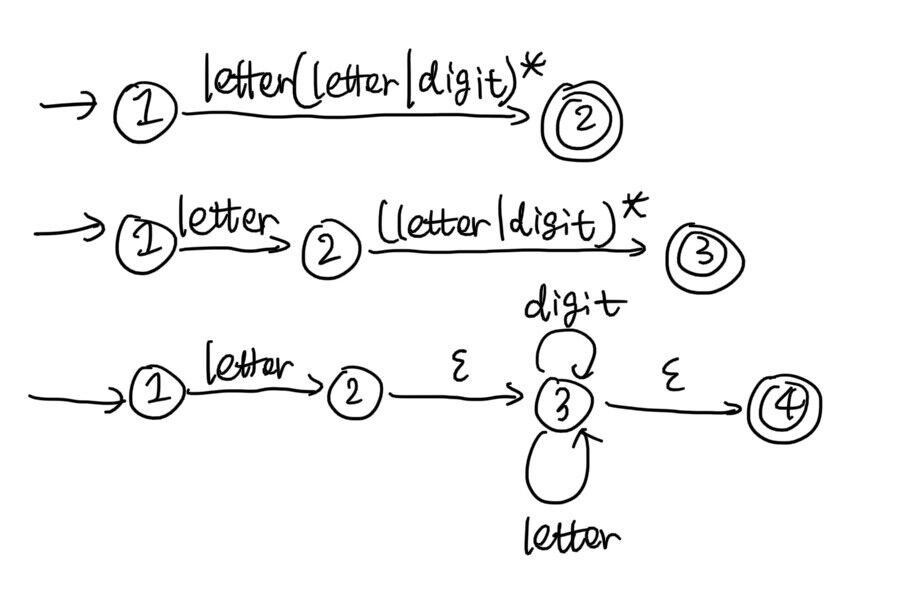
\includegraphics[width=0.6\linewidth]{figs/id001.png}
	\caption{标识符的非确定有限状态机推导过程}
	\label{fig: id001}
\end{figure}

\paragraph{NFA转化为DFA} 将最后得到的NFA确定化: 首先求DFA中的相应状态如表\ref{tab: id}

\begin{table}[H]
	\begin{center}
	\centering
	\caption{DFA中相应状态转化表}
	\label{tab: id}
	\begin{tabular}{|c|c|c|}
		\hline
		 & \textbf{letter} & \textbf{digit} \\
		\hline
		S0=(1) & (2,3,4) & - \\
		\hline
		S1=(2,3,4) & (3,4) & (3,4) \\
		\hline
		S2=(3,4) & (3,4) & (3,4) \\
		\hline
	\end{tabular}
	\end{center}
\end{table}

根据状态转换表得到相应的DFA如\ref{fig: id002}所示

\begin{figure}[H]
	\centering
	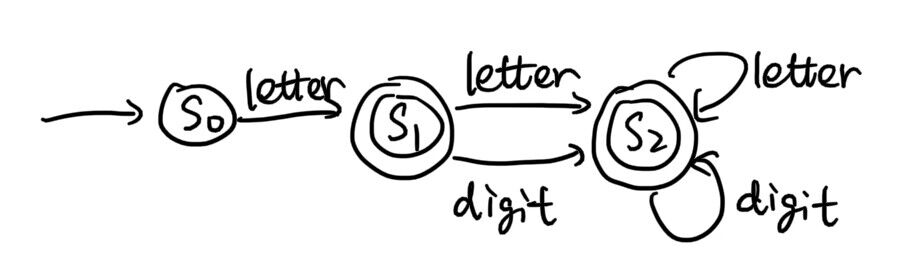
\includegraphics[width=0.5\linewidth]{figs/id002.png}
	\caption{标识符对应的DFA}
	\label{fig: id002}
\end{figure}

该DFA可以经过最小化后得到\ref{fig: id003}所示的最小化DFA

\begin{figure}[H]
	\centering
	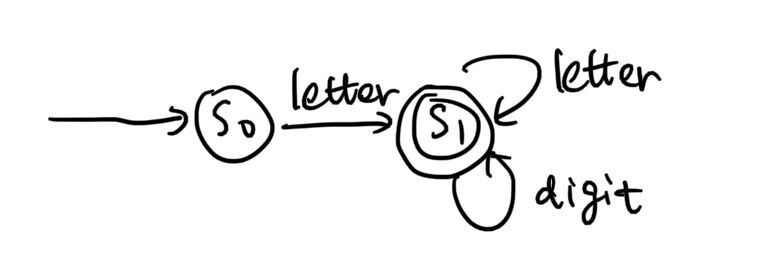
\includegraphics[width=0.01\linewidth]{figs/id003.png}
	\caption{标识符对应的最小化DFA}
	\label{fig: id003}
\end{figure}

\subsubsection{无符号数常量的正规文法, 正规式, NFA和DFA}

\paragraph{正规文法和正规式}

\begin{lstlisting}
	digits -> digit digit*
\end{lstlisting}

\paragraph{正规式转化为NFA}

\paragraph{NFA转化为DFA}

\subsubsection{四则运算的正规文法, 正规式, NFA和DFA}

\paragraph{正规文法和正规式}

\begin{lstlisting}
	expr -> expr (+ | -) term | term
	term -> term (* | /) factor | factor
	factor -> (expr) | digits | identifier	
\end{lstlisting}

\paragraph{正规式转化为NFA}

\paragraph{NFA转化为DFA}

\subsubsection{关系运算的正规文法, 正规式, NFA和DFA}

\paragraph{正规文法和正规式}

\begin{lstlisting}
	uneqExpr -> expr | uneqExpr < assignExpr | uneqExpr > assignExpr
	eqExpr -> expr | uneqExpr = assignExpr | uneqExpr ! assignExpr
	assignExpr -> expr | = expr
\end{lstlisting}

\paragraph{正规式转化为NFA}

\paragraph{NFA转化为DFA}

\subsubsection{\lstinline|/**/|型注释的正规文法, 正规式, NFA和DFA}

\paragraph{正规文法和正规式}

\begin{lstlisting}
	cmt -> / cmtStart
	cmtStart -> \* doc
	doc -> [^\*]* doc | \* cmtEnd
	cmtEnd -> \* cmtEnd | [^\*/] doc | /
\end{lstlisting}

\paragraph{正规式转化为NFA}

\paragraph{NFA转化为DFA}

\section{词法分析程序}

\section{测试}

\section{实验总结}

\end{document}